\chapter{Estado del Arte}\label{chapter:state-of-the-art}

\section{Sistemas, Modelos y Simulación}

Todo problema tiene un dominio en el cual se presenta y exige la construcción de un sistema, es decir, la selección y/o definición de entidades (mediante propiedades), relaciones estructurales y relaciones funcionales (entre estas entidades), las que se consideran involucradas y relevantes a la solución del problema. \parencite{temasdesimulacion} \\

Los sistemas se convierten en objeto de investigación para resolver el problema y se construyen y reconstruyen en varios niveles de abstracción según un proceso denominado modelación que suministra a diferentes niveles de abstracción representaciones estructurales y funcionales a las que se denomina modelos del sistema. El objetivo de crear modelos de un sistema tiene como fin esencialmente observar y/o modificar y/o controlar en condiciones ideales su conducta o dinámica. \parencite{temasdesimulacion} \\

La simulación es el proceso mediante el cual los procesos (dinámica) de un sistema son observados y/o modificados y controlados mediante modelos apropiados a tales fines. La dinámica de un sistema se considera simulada sólo en la medida en que esta dinámica, mediante su observación controlada, puede ser modificada con vistas a verificar principios o leyes y/o a determinar su forma más satisfactoria de realización. Siendo la computadora es el instrumento ideal para tales fines la simulación es esencialmente computacional. \parencite{temasdesimulacion} \\

De manera muy simple podemos decir que un sistema es  “[…] un conjunto de elementos relacionados entre sí y que funcionan como un todo”. \parencite{noauthor_simulacion_nodate} \\

\subsection{Sistema}

Según  \parencite{temasdesimulacion}, un sistema esta constituido por estructuras y procesos de un dominio de un problema las cuales se obtienen por abstracción a partir del dominio orientada por el problema.\\

A modo general existen varios tipos de sistemas, entre estos podemos mencionar los sistemas naturales, que están constituidos por estructuras y funciones de la realidad (átomos, partículas, sistemas biológicos); los sistemas socio-políticos, que son producto del desarrollo histórico, político y social (países, comunidades, sociedades); por último existen los denominados sistemas tecnológicos, resultado de la invención del hombre (máquinas, computadoras, sistemas eléctricos).\\

\subsubsection{Sistemas Dinámicos}

Los sistemas dinámicos son aquellos que tienen en cuenta el tiempo como dimensión fundamental y necesaria para describir su estructura, así como sus procesos. Existen dos tipos de sistemas dinámicos:
\begin{itemize}
	\item Sistema dinámico estacionario: la estructura del sistema no cambia y los procesos ocurren en el tiempo pero no se considera la dependencia del tiempo.
	\item Sistema dinámico no-e	stacionario: la estructura del sistema cambia con el tiempo y los procesos del sistema ocurren en y dependen del tiempo. \parencite{temasdesimulacion}
\end{itemize}

En esta investigación se trabajará con sistemas dinámicos a menos que el autor indique lo contrario.\\

\subsubsection{Sistema y Medio}

Un sistema existe (funciona, se desarrolla, interactúa) en un medio (ambiente). Medio es un sistema en el cual actúa, funciona, se desarrolla, con el cual interactúa en general un sistema bajo estudio. \parencite{temasdesimulacion}\\

Un sistema se considera cerrado si no se le asocia un medio, de lo contrario se le considera abierto. \parencite{temasdesimulacion}\\ Este se relaciona con su medio mediante entradas y salidas y a su vez este cambia en dependencia a su interacción con su medio.
No podemos dejar de mencionar el concepto de estado del sistema, que no es más que quien se encarga de almacenar lo mas importante de los estos cambios.
En general la acción del medio sobre un sistema (entrada) y el estado de este último son parámetros necesarios para predecir su comportamiento (estado) futuro y/o su salida o respuesta al medio. Luego, la dinámica de un sistema se describe en términos de una función de cambio de estado y una función de emisión de salida. \parencite{temasdesimulacion}\\

\subsubsection{Sistemas deterministas, no-deterministas y aleatorios}

Los sistemas se pueden distinguir en dependencia de la información que tengamos de estos, sea conocida, desconocida o parcialmente conocida (sistemas con información completa o incompleta).
Según lo anterior, un sistema se puede considerar determinista si los últimos estados de este se derivan de los anteriores o están determinados por ellos; por otra parte, se tienen los sistemas estocásticos o aleatorios en el que los estados futuros no están determinados por los anteriores.
Si un sistema es determinista, esto no implica necesariamente que los estados posteriores del sistema sean predecibles a partir del conocimiento de los anteriores. \parencite{darling_deterministic_nodate}

\subsection{Modelo}

Precisar cuáles entidades del sistema intervienen de algún modo en el problema que se desea resolver y las relaciones causales que influyen en su comportamiento y en el del sistema en su conjunto, conduce a un proceso de simplificación de la realidad, de abstracción, que se conoce como modelación.
Diferentes problemas sobre un mismo dominio da lugar a la concepción de diferentes sistemas sobre el mismo.\\

Los sistemas creados para solucionar un problema deben ser observables y/o controlables y/o modificables, o sea dado un sistema creado para resolver un problema se desea Observarlo y/o Controlarlo y/o Modificarlo. \parencite{temasdesimulacion}\\

Un modelo se utiliza para poder observar, controlar y modificar un sistema. Por lo tanto podemos definir un modelo como una descripción abstracta de un sistema que representa de forma aproximada su comportamiento.
Según \parencite{temasdesimulacion}, “Un modelo es un sistema que representa a otro sistema.”\\

Gran parte de los sistemas reales dificultan mucho que dicho modelo sea observable, controlable y modificable.\\

Podemos catalogar los modelos en dependencia de su estructura, entre estos tenemos los modelos del sistema real, a escala, analógico, matemático, computacional. En este último centraremos nuestra atención.\\

\subsubsection{Modelado Computacional}
El modelado computacional es el uso de computadoras para simular y estudiar sistemas complejos utilizando las matemáticas, la física y la informática. Un modelo computacional contiene numerosas variables que caracterizan el sistema bajo estudio. La simulación se realiza ajustando las variables, solas o combinadas, y observando los resultados. El modelado computacional permite a los científicos realizar miles de experimentos simulados por computadora. Los miles de experimentos por computadora identifican los pocos experimentos de laboratorio que tienen más probabilidades de resolver el problema bajo estudio. \parencite{noauthor_modelado_nodate}

Los modelos computacionales de hoy en día pueden estudiar sistemas muy complejos, y un caso particular de esto seria nuestro objeto de estudio, un \textbf{sistema de cultivos}, siendo este un sistema abierto, dinámico no estacionario, determinista en cierto punto con una gran porción de aleatoriedad e información la mayoría de veces incompleta. \\

\subsection{Simulación}
La simulación puede verse como la ejecución, observación y cambio de un modelo determinado.
Según la definición de Robert E. Shannon, \parencite{shannon1975simulacion} la simulación es el “[…] proceso de diseñar y desarrollar un modelo computarizado de un sistema o proceso y conducir experimentos con este modelo con el propósito de entender el comportamiento del sistema y/o evaluar varias estrategias con las cuales se puede operar el sistema”.\\

En las ciencias, la simulación es el artificio contextual que referencia la investigación de una hipótesis o un conjunto de hipótesis de trabajo utilizando modelos.
Simulación es una técnica numérica para conducir experimentos en una computadora digital. Estos experimentos comprenden ciertos tipos de relaciones matemáticas y lógicas, las cuales son necesarias para describir el comportamiento y la estructura de sistemas complejos del mundo real a través de largos periodos de tiempo. \parencite{noauthor_simulacion_nodate}\\

La simulación computacional es la basada en modelos computacionales.

Los recientes avances en las metodologías de simulación y la gran disponibilidad de diversos tipos de software existentes en el mercado han hecho que la técnica de simulación sea una de las herramientas más ampliamente usadas en el \textbf{análisis de sistemas}.

Gracias a los avances tecnológicos una computadora puede tomar el papel de cualquier máquina o sistema existente. A medida que aumenta la complejidad del sistema mas se dificulta para la computadora replicar dicho comportamiento, por lo tanto es necesario emplear modelos del sistema simplificado, tomando solo de este lo que sea relevante para el análisis.

\subsubsection{Modelado de sistemas complejos}

En la actualidad, debido a los avances tecnológicos del microprocesador, han nacido nuevas técnicas de modelado de sistemas complejos, entre estas podemos mencionar dos grandes exponentes que son la simulación basada en agentes y la dinámica de sistemas. Ambas complementan modelos no formales de sistemas complejos y modelos matemáticos con un mayor nivel de abstracción.\\

Varios filósofos como Hesse \parencite{echenique1970models} y Hughes \parencite{hughes1997models} proponen un esquema general del proceso científico. Estos modelos se construyen para desarrollar procesos de inferencia sobres algunos aspectos de sistemas reales observados con anterioridad. Tomando como base estos procesos de inferencia se mejora la forma de entender los sistemas reales observados. \parencite{izquierdo2008modelado}

En la figura (\ref{fig:img_1}) se muestra el proceso de creación y uso de un modelo.

\begin{figure}[!h]
	\centering
	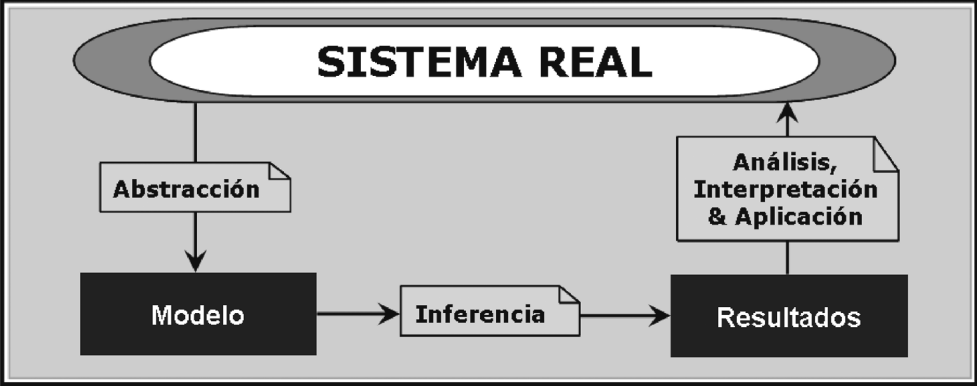
\includegraphics[scale=0.5]{Images/esquema_modelado_cientifico.png}
	\caption{Esquema general del proceso de modelado científico. \parencite{izquierdo2008modelado}}
	\label{fig:img_1}
\end{figure}

Se puede concluir que luego de analizar un modelo, se llegaran a conclusiones que no serán estrictamente rigurosas respecto a lo que sucede en el sistema real. Sin embargo, con la aplicación del modelo se obtendrán conocimientos que sin esta no hubiese sido posible adquirir.\\

Como se observa en la figura (\ref{fig:img_1}), el proceso de modelado no es unidireccional ya que generalmente se suele diseñar un modelo, del cual se obtienen resultados, teniendo en cuenta estos se perfecciona el modelo mediante ciertos cambios lógicos en sus valores iniciales o intermedios. El modelo inicial puede haber fallado por dos motivos fundamentales:
\begin{itemize}
	\item porque no parecieran derivarse lógicamente de las premisas del modelo (proceso de verificación).
	\item porque, aún siendo lógicamente correctos, difirieran excesivamente de los resultados observados en el sistema real que se está modelando (proceso de validación). \parencite{izquierdo2008modelado}
\end{itemize}

De una manera un tanto informal, podríamos decir que verificar consiste en valorar si el modelo que tenemos es correcto, mientras que validar consiste en estudiar si tenemos el modelo correcto.\\


Los sistemas complejos (p. ej. organismos pluricelulares, colonias de hormigas, ecosistemas, economías, sociedades…) están caracterizados por tener una estructura compuesta por varios niveles. En estos sistemas complejos \parencite{vicsek2002complexity, gilbert2004agent}:

\begin{itemize}
	\item Los componentes de niveles jerárquicos inferiores suelen mostrar un grado de autonomía significativo.
	\item El comportamiento del sistema surge a partir de la auto-organización de sus componentes, sin que esta organización esté controlada ni dirigida por ningún ente exterior al sistema.
	\item Los componentes básicos de estos sistemas complejos (células, hormigas, individuos, poblaciones, empresas…) perciben su entorno y responden a cambios en él de forma potencialmente diferente.
\end{itemize}

Todas estas características hacen que el proceso de modelado formal de sistemas complejos difiera sustancialmente del de otros sistemas más simples. En particular, su naturaleza descentralizada, la presencia de bucles de causalidad y retroalimentación no lineales, y el hecho de contener varias unidades más o menos autónomas, que pueden interaccionar, evolucionar, y adaptar su comportamiento a cambios en el entorno, implica que en la mayoría de los casos es muy difícil, si no imposible, conseguir un modelo que pueda describir el sistema complejo adecuadamente y que además sea resoluble matemáticamente. \parencite{izquierdo2008modelado}\\

Un modelo computacional es un modelo formal (que por lo tanto puede expresarse en lenguaje matemático como un conjunto de ecuaciones), y la simulación computacional es una herramienta que nos permite estudiarlo más allá de los límites actuales de las matemáticas. De este modo, el resultado final es un modelo potencialmente más realista, y que todavía conserva el rigor formal de los modelos matemáticos más tradicionales. \parencite{izquierdo2008modelado}\\

Luego de analizada la posibilidad de trabajar con modelos formales de mayor complejidad, se hace necesario ampliar el esquema visto en la figura (\ref{fig:img_1}) a la siguiente (\ref{fig:img_2}):

\begin{figure}[!h]
	\centering
	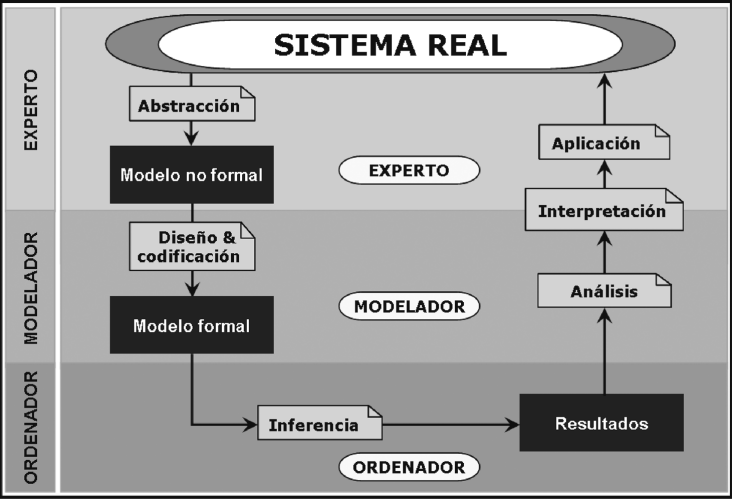
\includegraphics[scale=0.5]{Images/esquema_modelado_cientifico_con_abstraccion.png}
	\caption{Proceso de modelado con abstracción intermedia. \parencite{izquierdo2008modelado}}
	\label{fig:img_2}
\end{figure}

\subsubsection{Simulación basada en agentes}

La simulación basada en agentes (agent-based modelling) es un novedoso método de investigación para las ciencias sociales. Dicho método fue inicialmente desarrollado en el campo de la IA (Inteligencia Artificial) a lo largo de la década de los 50 del pasado siglo y ha sido empleado desde entonces para resolver algunos de los problemas propios de las ciencias físicas y naturales. Sin embargo, ha empezado a utilizarse recientemente en las ciencias sociales, aunque su objeto de estudio difiera de los de las ciencias físicas y naturales. \parencite{garcia2016simulacion}\\

Mediante la simulación basada en agentes, el modelador reconoce
explícitamente que los sistemas complejos, y en particular los sociales, son
producto de comportamientos individuales y de sus interacciones. \parencite{izquierdo2008modelado}
Este tipo de simulación se distingue de de otras por la forma en que se construye la primera abstracción del sistema real y por tanto del modelo formal.\\

Se caracterizan por comprender varios agentes que son, en mayor o menor grado, autónomos, heterogéneos e independientes, que muestran cada uno sus propias metas y objetivos, y que generalmente son capaces de interaccionar entre sí y con su entorno \parencite{torsun1995foundations}. En muchas ocasiones, pero no siempre, son sistemas caracterizados por la existencia de un número grande de agentes relativamente simples, que pueden evolucionar a lo largo del tiempo para adaptarse a nuevas condiciones del entorno o a nuevos objetivos. \parencite{izquierdo2008modelado}

A continuación se pueden ver los cuatro tipos básicos de agentes encontrados en casi todos los sistemas inteligentes:
\begin{itemize}
	\item Agentes reactivos simples: son el tipo de agente más sencillo. Estos agentes seleccionan las acciones sobre la base de las percepciones actuales, ignorando el resto de las percepciones históricas.
	\item Agentes reactivos basados en modelos: La forma más efectiva que tienen los agentes de manejar la visibilidad parcial es almacenar información de las partes del mundo que no pueden ver. O lo que es lo mismo, el agente debe mantener algún tipo de estado interno que dependa de la historia percibida y que de ese modo refleje por lo menos alguno de los aspectos no observables del estado actual.
	\item Agentes basados en objetivos: El conocimiento sobre el estado actual del mundo no es siempre suficiente para decidir qué hacer. En otras palabras, además de la descripción del estado actual, el agente necesita algún tipo de información sobre su meta que describa las situaciones que son deseables.
	\item Agentes basados en utilidad: Las metas por sí solas no son realmente suficientes para generar comportamiento de gran calidad en la mayoría de los entornos. Las metas sólo proporcionan una cruda distinción binaria entre los estados de «felicidad» y «tristeza», mientras que una medida de eficiencia más general debería permitir una comparación entre estados del mundo diferentes de acuerdo al nivel exacto de felicidad que el agente alcance cuando se llegue a un estado u otro. Como el término «felicidad» no suena muy científico, la terminología tradicional utilizada en estos casos para indicar que se prefiere un estado del mundo a otro es que un estado tiene más utilidad que otro para el agente. \parencite{russell2004inteligencia}
\end{itemize}
Puesto que el énfasis en la simulación basada en agentes está en encontrar abstracciones apropiadas que describan los componentes básicos del sistema y sus interacciones (en vez de buscar abstracciones que versen directamente sobre la dinámica global del sistema), esta técnica de modelado es particularmente útil para modelar procesos emergentes de forma natural.\parencite{izquierdo2008modelado}

\subsubsection{Simulación basada en dinámica de sistemas}

La dinámica de sistemas, situada en la misma área de conocimiento que la teoría general de sistemas, la automática y la cibernética, nació de la aplicación —realizada en la década de los 50 por Jay W. Forrester, de la teoría de los bucles de realimentación a un caso concreto de gestión industrial. Aplicada en 1970 al estudio del mundo como sistema dinámico,  esta metodología, cuyo objetivo es construir modelos dinámicos de sistemas sociales basándose en la opinión de expertos y el uso de la simulación con computadores, es actualmente una  herramienta que cubre un amplio campo de aplicaciones, desde la  gestión de empresas hasta la construcción de modelos urbanos, regionales, sociológicos y ecológicos. \parencite{aracil1997dinamica} \\

La dinámica de sistemas es otra técnica de modelado de sistemas complejos. También se utiliza para modelar sistemas en ingeniería \parencite{ford1997system, ford1998dynamic}, economía y negocios \parencite{bayer2004sterman, ellis2007impacto}, entre otros. \parencite{izquierdo2008modelado}.

Esta tiene como base el concepto de retroalimentación, o causalidad circular entre variables observables.
A diferencia de la simulación basada en agentes, el centro de la dinámica de sistemas está en la relación que existe entre las variables observables.
Por tanto la idea central de este modelo de simulación está en encontrar las variables críticas del sistema complejo e identificar los vínculos causales existentes entre ellas.

\section{Modelos de Simulación de Cultivos}

Los modelos de simulación son una herramienta fundamental para entender la complejidad de los sistemas ecológicos y ambientales como bien se plasmó anteriormente.
Un buen modelo es capaz de revelar interacciones entre los diferentes componentes que no eran evidentes al estudiar cada uno de los procesos separadamente y permitirá llevar a cabo experimentos, que no se podrían realizar en el sistema real dado que pueden ser muy costosos en términos de trabajo, recursos o tiempo.
Sin perder generalidad, una de las funciones que estos permiten, es la de analizar, pronosticar e incluso mejorar el rendimiento de los cultivos.
Dichos modelos tienen varias aplicaciones potenciales en la actualidad en respuesta a temas que guardan relación con la investigación, manejo y planificación de cultivos. Estos juegan un papel importante en la toma de decisiones en la agricultura al cuantificar, interpretar y predecir las necesidades hídricas de los cultivos, su desarrollo y rendimiento. \parencite{granmaEMFord}
Durante las últimas décadas se han aplicado estos modelos en países de clima templado debido a los grandes beneficios que aportan.\\

Como un modelo no es más que una representación simplificada de un sistema, y un sistema es una parte bien delimitada de la realidad, se puede ver un sistema de cultivo como el cultivo en sí con todos sus órganos, o sea, raíz, tallo y hojas, sus procesos y mecanismos como el crecimiento, desarrollo, fotosíntesis, transpiración, entre otros. \parencite{hernandez2009modelos}

La modelación empezó a aumentar su importancia en el sector de la agronomía dada su capacidad de brindar información de manera periódica de todo el sistema biológico o una parte, como es el sistema de producción agrícola. \parencite{guevara2007simulacion}

Una sabia utilización de los recursos en la actualidad implica una mayor probabilidad de aumento de la producción alimenticia. Además, el cambio climático, la variabilidad del clima, suelo, el secuestro de carbono a largo plazo, efectos en la seguridad alimentaria y la sostenibilidad del medio ambiente se han convertido en aspectos importantes a tener en cuenta. Por otra parte, la agricultura de los países tropicales enfrenta cada vez más nuevos retos, debido a cambios en las políticas macroeconómicas, al crecimiento de la población, el bajo rendimiento y a los límites de sostenibilidad de los recursos naturales utilizados en la producción. Conocer adecuadamente la dinámica y los efectos de los principales factores involucrados en el desarrollo agrícola, para poder elaborar alternativas viables de progreso en nuestros trópicos americanos, conservando los recursos naturales mediante su utilización racional, son aspectos de especial importancia y deben ser objeto prioritario de actualización profesional. Cada día resulta más crucial la necesidad de la información en la toma de decisiones y existe un vacío importante entre la información que se necesita y la que se genera tradicionalmente mediante la investigación disciplinaria. Para este propósito una herramienta como los \textbf{modelos de simulación de los cultivos} es de gran utilidad.  \parencite{hernandez2009modelos}

Los modelos de simulación son una herramienta que facilitan la toma de decisiones, para seleccionar la mejor alternativa que se puede lograr con una combinación de recursos y precios, y muestra cuánto se podría pagar por una unidad más de cada recurso que se agota. \parencite{holmann2002uso}\\

En la década del 50 aparecen los modelos de simulación, luego a mediados de los 60 aparece el concepto de sistemas dinámicos, que como se vio en anteriores secciones, incluyen la variable tiempo y representan el flujo de esos procesos y sus interacciones. En esta última etapa, destacan dos importantes pioneros, W. G. Duncan en la University of Kentucky y C. T. de Wit en la Agricultural University de Wageningen, que desarrollaron modelos como herramienta para explicaciones científicas, como por ejemplo, sintetizar y mejorar la comprensión de procesos tales como la intercepción de radiación y fotosíntesis, desarrollando modelos simples que consideraban únicamente la producción potencial relacionada con la radiación y la temperatura. En la década del 70 se formaliza aquel concepto de dinámica de sistemas y en los 80 se refina mediante técnicas de computación la verificación, validación y evaluación de esos modelos. 
En esta última década aparecen los primeros modelos de simulación para los cultivos de maíz, soja, trigo y arroz, incluidos en el paquete DSSAT (Decision Support System for Agrotechnology Transfer) “Sistema de apoyo para las decisiones de transferencia agrotecnológica”.
La simulación de sistemas agrícolas comenzó a ser una herramienta fundamental para la integración de los diferentes componentes productivos dentro de los sistemas agrícolas. \parencite{hernandez2009modelos}

Los avances en el conocimiento de las interacciones dentro del ecosistema, influenciado por el ambiente y por las prácticas de manejo, expandió la potencialidad de uso de esta herramienta como ayuda para la toma de decisiones. \parencite{barrett2018humanization}

A mediados de los 90 gana auge la tecnología informática permitiendo una mayor utilización de estos modelos para el estudio y resolución de problemas específicos como el desarrollo y crecimiento de los cultivos, evaluación de respuesta a la fertilización, estrategias de riego, situaciones de estrés, predicción de pérdidas por erosión, lixiviación de pesticidas, contaminación del ambiente, calentamiento global de la atmósfera, entre otros. \parencite{guevara2007simulacion}

En general, son aceptables los puntos de vista de los que aseveran que la implementación de los modelos de simulación para las ciencias agrícolas y biológicas y sus usos prácticos está en un momento de gran importancia. \parencite{galvez2008modelacion}

\subsection{Modelos, Características y su Utilización}

En la actualidad se cuenta con una rica fuente de datos y conocimiento dentro de cada campo en particular, debido a esto se desarrollan modelos con distintos niveles de complejidad. La clasificación de los modelos ha sido intentada anteriormente, pero no se pueden hacer delimitaciones definidas, ya que los modelos generalmente poseen características de más de un grupo. \parencite{galvez2008modelacion, hernandez2009modelos}\\

Se pueden clasificar estos modelos de simulación en dos grupos:
\begin{enumerate}
	\item Empíricos: son descriptivos, se derivan de datos observados sin involucrar procesos fisiológicos y tienen escasa capacidad explicativa.
	\item Mecanicistas: poseen capacidad explicativa de la fisiología del cultivo, porque consideran aspectos como la temperatura, la radiación fotosintéticamente activa, el índice de área foliar, la fotosíntesis, la respiración y la eficiencia en el uso de la radiación. \parencite{refugio2004modelos}
\end{enumerate}

Dentro de estas clasificaciones existen otras categorías, que de acuerdo a sus características han sido nombradas de diferente forma.
Los modelos que estudian las relaciones biológicas para describir el comportamiento de un sistema son denominados modelos mecanísticos, a diferencia de los modelos empíricos que describen las relaciones matemáticas entre los datos. \parencite{vargas2004modelo}.

\textbf{Modelos empíricos o descriptivos}: Estos modelos describen, de un modo simplificado, el comportamiento de un cultivo.
El desarrollo de un modelo empírico se basa en la individualización, a partir de datos experimentales, de una o más ecuaciones matemáticas, para la representación del proceso examinado. Las principales carencias de este tipo de aproximación son las de investigar en la limitada validez en ambientes diversos a los originales y en el empleo de las ecuaciones que a menudo no tienen un significado biológico \parencite{bandi2003instrumentos}

Los modelos empíricos son descripciones directas de los datos observados y se expresan generalmente como ecuaciones de regresión (con uno o varios factores) y se utilizan para estimar la producción final. Ejemplos de tales modelos incluyen la respuesta de la producción a la aplicación de fertilizantes, la relación entre el área de la hoja y la cantidad de hojas de una planta dada, la relación entre la altura del tallo y el número de tallos, su diámetro y la producción final de caña de azúcar. \parencite{galvez2008modelacion}

\textbf{Modelos mecanísticos}: Estos modelos son aquellos que describen el comportamiento del sistema en términos de propiedades de bajo nivel. Por tanto, existe comprensión o explicación en los niveles inferiores. Estos modelos tienen la habilidad de imitar importantes procesos físicos, químicos o biológicos, y describir cómo y por qué resulta una respuesta particular. El analista comienza usualmente con algún empirismo y en la medida que se gana en conocimiento se introducen variables y parámetros adicionales para explicar la producción de la cosecha. Así, el analista adopta un enfoque reduccionista. La mayoría de los modelos de crecimiento de cultivos caen dentro de esta categoría. \parencite{galvez2008modelacion}

\textbf{Modelos estáticos y dinámicos}: Los modelos estáticos representan relaciones entre las variables que no se modifican en el tiempo y, por tanto, se conoce su valor final y no su evolución en el tiempo (por ejemplo la simulación de la intercepción solar, fotosíntesis). \parencite{bandi2003instrumentos}

Los modelos dinámicos describen el modo en el cual el sistema cambia en el tiempo y, por lo tanto, es posible seguir la evolución temporal de cada una de las variables del sistema (por ejemplo el balance de nitrógeno y agua en el suelo). \parencite{bandi2003instrumentos}

\textbf{Modelos determinísticos y estocásticos}: Los modelos determinísticos atribuyen un solo valor a cada variable del sistema. \parencite{bandi2003instrumentos} Hacen predicciones para cantidades (por ejemplo, producción de la cosecha) sin ninguna distribución probabilística asociada, varianza o elemento aleatorio. En los sistemas biológicos y agrícolas son normales las variaciones, debido a imprecisiones en los datos recogidos y a heterogeneidad del material con que se ha trabajado. En algunos casos, los modelos determinísticos pueden ser adecuados a pesar de estas variaciones inherentes, pero en otros pueden resultar insatisfactorios, por ejemplo, en la predicción de lluvia. Cuanto mayor sea la incertidumbre del sistema, más inadecuados se vuelven los modelos determinísticos. \parencite{galvez2008modelacion} Los modelos estocásticos señalan, en cambio, para una variable una distribución de valores. \parencite{bandi2003instrumentos}

Cuando la variación y la incertidumbre alcanzan un nivel alto, se hace recomendable desarrollar un modelo estocástico que dé un valor medio esperado con una varianza asociada. Sin embargo, los modelos estocásticos tienden a ser difíciles de manipular y rápidamente se vuelven muy complejos. Por consiguiente, es recomendable intentar resolver el problema inicialmente con un enfoque determinístico y utilizar el enfoque estocástico sólo si los resultados no son adecuados o satisfactorios. \parencite{galvez2008modelacion, hernandez2009modelos}

Para el procesamiento y análisis de la problemática, utilizando análisis de regresión, es necesario considerar \parencite{fernandez2003biomodelos, rodriguez2018aplicaciones}:
\begin{itemize}
	\item Ploteo de puntos para analizar tendencia de datos.
	\item Selección del tipo de modelo a ajustar.
	\item Ajuste del modelo, con el apoyo de un software apropiado.
	\item Descripción del proceso a partir del modelo obtenido.
\end{itemize}

En estos estudios se requiere de una labor eficiente en la organización y desarrollo de la investigación científica y el conocimiento que esta genera, a lo que puede contribuir en gran medida la aplicación consecuente de estos modelos, con el apoyo de las nuevas tecnologías de la información y la comunicación. Igualmente, con mucha frecuencia, no se valoran los supuestos teóricos de los modelos estadísticos y no se establecen conclusiones válidas a partir de la información analizada. \parencite{guerra2003criterios}:
\begin{itemize}
	\item Métodos de ajuste de los modelos.
	\item Error estándar de los estimadores de los parámetros (Test t de Student).
	\item Coeficiente de variación de los estimadores.
	\item Límites de confianza de los parámetros.
	\item Test de redundancia de los parámetros.
	\item Análisis de varianza relacionado con el modelo en cuestión.
	\item Coeficiente de determinación $R^2$ y $R^2$ ajustado por los grados de libertad, para modelos con diferentes números de parámetros.
	\item Suma de cuadrados o Cuadrado Medio Residual.
	\item Error estándar de estimación.
	\item Test de falta de ajuste del modelo.
	\item Análisis del efecto del uso de transformaciones en el modelo.
	\item Diagnóstico y tratamiento de la multicolinealidad, en modelos de regresión lineal múltiple.
	\item Validación de las predicciones del modelo.
	\item Estadístico PRESS (Suma de Cuadrados del Error de Predicción).
	\item Estadístico CMEP (Cuadrado Medio del Error de Predicción).
	\item Estadístico Cp de Mallows.
	\item Coeficientes de correlación entre los resultados predichos y los reales.
	\item Análisis de la precisión de las estimaciones.
	\item Análisis de los residuos.
	\item Normalidad (Test de ShapiroWilks, Kolmogorov-Smirnov).
	\item Autocorrelación (Test de Rachas, Signos, DurbinWatson, $X^2$ de independencia, Ljung y Box).
	\item Homocedasticidad (Gráficos de los residuos, Test de Cochran, Bartlett y Hartley).
\end{itemize}

\subsection{Aplicaciones de Modelos y Simulación de cultivos agrícolas en Cuba}

Desde la década de los 80 se ha venido utilizando la modelación por algunos investigadores cubanos con el objetivo de describir el crecimiento de cultivares. En el Instituto Nacional de Ciencias Agrícolas (INCA) se realizaron comparaciones entre varias funciones matemáticas para describir el crecimiento de algunos órganos en posturas de café crecidas en vivero \parencite{soto1986crecimiento}. Se determinó, además, la influencia del uso o no de la sombra durante el período de aviveramiento, la altura sobre el nivel del mar y dos fechas de siembra, en la dinámica de crecimiento de plántulas de cafeto \parencite{soto1991dlnamlca, hernandez2009modelos, rodriguez2018aplicaciones}.

También se han comparado modelos para medir la respuesta a dosis de nitrógeno en maíz y cafeto. Lo cual demostró que un modelo discontinuo rectilíneo resulta más adecuado en el sistema de recomendación de dosis óptimas de fertilizantes nitrogenados para estos cultivos, en comparación al modelo curvilíneo, que brinda dosis óptimas superiores, que implican un menor factor parcial de productividad de la dosis recomendada \parencite{martin2016comparacion, rodriguez2018aplicaciones}.

Otros trabajos aplicaron herramientas de modelación para el análisis de las respuestas de las interacciones planta-ambientemanejo en distintos escenarios de la producción de arroz, maíz, sorgo y trigo en Cuba \parencite{hernandez2016utilizacion}; demostrando que estas permiten establecer estrategias para el desarrollo de los cultivos estudiados en escenarios futuros y en otras condiciones de cultivo. Por primera vez en el país, se cuenta con información para poder predecir el comportamiento y rendimiento de estos cereales. Demuestran además que el modelo DSSAT puede ser utilizado para las condiciones de Cuba en los indicadores de rendimiento y sus componentes. \parencite{rodriguez2018aplicaciones}.

Por los beneficios que aportan los modelos determinísticos, especialistas de la Universidad Agraria de La Habana y del Instituto Nacional de Riego y Drenaje, elaboran los primeros trabajos para utilizar, en las condiciones geográficas de Cuba, cinco de los modelos agrohidrológicos de alcance internacional. Por primera vez en Cuba se brindan los parámetros que describen las propiedades hidráulicas para los principales grupos de suelos cubanos. Esta investigación le confiere validez al modelo SWACROP para ser utilizado en el cultivo de la papa en condiciones tropicales \parencite{ruiz1997utilizacion, rodriguez2018aplicaciones}.

Algunos trabajos se han realizado, durante varios años, en la evaluación y validación de diferentes modelos de simulación de transferencias hídricas para las condiciones edafoclimáticas de la región sur de La Habana (actualmente Mayabeque y Artemisa). Estas investigaciones pretenden resumir y discutir las principales características de los modelos de simulación STIC y MACRO y sus posibilidades para la predicción del comportamiento de los cultivos agrícolas ante diferentes manejos de agua, fertilización y ambientes climáticos. \parencite{lopez20143, robaina2013crop, rodriguez2018aplicaciones}

También se ha utilizado la modelación matemática con el fin de estudiar el crecimiento del diámetro medio, la altura media y el volumen por hectárea de \textit{Pinus caribaea morelet var.}
\textit{Caribaea barret} y \textit{golfari }en la Unidad Silvícola “Los Jazmines” de Viñales y en la Empresa Forestal Integral “La Palma” \parencite{suarez2011modelacion, sarria2013modelacion}. Donde se determinaron los modelos que mejor describen el comportamiento de las variables estudiadas en cada uno de los escenarios. \parencite{rodriguez2018aplicaciones}

La aplicación a la producción de pastos y forrajes, tuvo sus inicios en pasto estrella (C. nlemfuensis) \parencite{del1998analisis, torres1999empleo}, donde se encontraron relaciones polinómicas entre las variables; pero en estos modelos los parámetros no tienen interpretación biológica. Posteriormente se modeló y simuló el comportamiento productivo del pasto estrella (C. nlemfuensis) bajo diferentes frecuencias de corte, niveles de fertilización y condiciones climatológicas adversas para el desarrollo de este cultivo \parencite{rodriguez2020modelacion}. El modelo Gompertz utilizado ajustó los datos con coeficientes de determinación que estuvieron alrededor del $99 \% $ para los períodos lluvioso y poco lluvioso. Además pronostica que un incremento de la temperatura media del planeta en 2 y 4 ºC afectará el rendimiento de materia seca acumulada de este cultivo principalmente en el período poco lluvioso. \parencite{rodriguez2018aplicaciones}

Otros autores estudiaron la dinámica de acumulación de biomasa del king grass (P. purpureum) o de algunos de sus clones con el empleo de modelos no lineales \parencite{diaz2007evaluacion, noda2013modelacion}. Además, en cultivares de Brachiaria, Panicum y Pennisetum y en variedades de Tithonia diversifolia, se evaluaron diferentes modelos y encontraron ajustes lineales para las variables en estudio \parencite{ramirez2012rendimiento, torres2012utilizacion, rodriguez2018aplicaciones}.

\subsection{Modelos de Cultivo más Conocidos}

Los modelos de simulación agronómica son herramientas que integran información, y permiten analizar y cuantificar las relaciones existentes entre los factores mencionados y sus efectos como componentes del sistema, para evaluar diferentes planteos productivos o analizar un factor manteniendo los otros constantes; por ejemplo, la variación del rendimiento por efecto del clima sin modificar el manejo, el genotipo y el suelo. Numerosos modelos han sido desarrollados por diferentes grupos de trabajo y cada uno de ellos tiene fortalezas y debilidades para predecir las variables de respuesta. Es por ello necesario validar los modelos en los ambientes en donde se utilizarán \parencite{salvagiotti2003analisis}.

No obstante la capacidad relativa de los modelos existentes y la credibilidad de sus resultados es todavía un aspecto importante a valorar. Esto está asociado primeramente a la no disponibilidad de datos apropiados para la validación del modelo y, por otra, a la inadecuación en las representaciones de los procesos e interacciones del sistema agua-suelo-planta-atmósfera. Es por tanto muy importante antes de adoptar uno u otro modelo para aplicaciones agrícolas y medioambientales que se realice un trabajo de evaluación y validación exhaustivo de estos \parencite{lopez20143}.\\

\textbf{DSSAT}: (Sistema de Apoyo de Decisiones para la Transferencia de la Agrotecnología). Desde 1983, un grupo internacional de científicos cooperantes han desarrollado modelos de simulación de cultivos, enfocados a proporcionar estimaciones realistas del comportamiento de los cultivos bajo diferentes estrategias de manejo y condiciones ambientales. Estos modelos se han combinado en un paquete, como parte de un programa de enlaces (software shell) conocido como Sistema de Apoyo para Decisiones de Transferencia de Agrotecnología (DSSAT, por sus siglas en inglés) \parencite{jones1998decision}.
Los modelos de simulación de cultivos del DSSAT utilizan archivos de datos para clima, suelo y manejo del cultivo. Estos archivos se utilizan para proveer en la simulación un ambiente parecido a donde crece el cultivo. El DSSAT, además, incluye varios programas de aplicación para análisis estacionales \parencite{thornton1994computer}, rotación de cultivo y análisis secuencial \parencite{thornton1995computer}, y análisis espacial a escala de campo o regional \parencite{engel1997aegis, thornton1997computer}. Los modelos proveen una de las mejores aproximaciones del comportamiento de los cultivos, integrando nuestro entendimiento de los procesos complejos de las plantas influenciados por el clima, el suelo y las condiciones de manejo \parencite{white2003gene}.
El modelo DSSAT ha sido usado por investigadores de todo el mundo en los últimos 15 años; este paquete tiene incorporado 16 modelos de cultivos diferentes, con un software que facilita la evaluación y aplicación de estos modelos de cultivos para diferentes propósitos \parencite{jones2003dssat}. Estos permiten simular el crecimiento de cultivos de importancia económica y han demostrado alta confiabilidad en distintas condiciones de clima, suelo y manejo \parencite{jones1993decision}. Con este modelo es posible organizar y archivar bases de datos sobre clima, suelos, cultivos, experimentos y precios; simular producciones de cultivo en una o varias épocas y en secuencias; analizar resultados y representar gráficamente simulaciones; analizar variabilidad espacial y evaluar diferentes prácticas de manejo específicas a una explotación o parte de ella \parencite{giraldo2007adaptacion}.\\

\textbf{UNSAT}: El software UnSat Suite Plus combina los modelos HELP, PESTAN, SESOIL, VLEACH y VS2DT en un nuevo ambiente gráfico de gran alcance, diseñado específicamente para simular el flujo del agua subterránea y el transporte unidimensional del contaminante con la zona no saturada. Este modelo unidimensional simula el flujo vertical descendente de aguas subterráneas, así como la migración de contaminantes disueltos en aguas subterráneas, a través de una fina columna de suelo.

El paquete de software UnSat Suite Plus incluye numerosas herramientas y elementos de diseño que le permitirán producir simulaciones de flujo profesionales. Las funciones de este producto incluyen:

\begin{itemize}
	\item Entorno de modelado unificado.
	\item Nuevo asistente de proyectos.
	\item Gestión de proyectos.
	\item Datos de entrada.
	\item Visualización gráfica.
	\item Enlaces de la base de datos.
	\item SWS Weather Generator.
	\item Integración perfecta.
	\item Presentación de resultados.
	\item Generador de informes automático.
\end{itemize}

Las funciones de simulación se posibilitan gracias a la integración de 5 modelos diferentes dentro del software de UnSat Suite plus. Estos modelos que se integran son:
\begin{itemize}
	\item HELP, es un modelo aplicable a los procesos hidrológicos de taludes, terraplenes, desmontes, laderas modificadas, etc., permitiendo comprobar la estabilidad, viabilidad y correcto diseño del mismo. También es eficaz en el cálculo del valor de la recarga del agua subterránea.
	\item PESTAN (PESTticide ANalítico), es un modelo analítico de pesticidas, que utiliza una solución analítica para predecir el transporte de solutos orgánicos con la zona no saturada a la tabla del agua subterránea. Resulta útil para evaluar el potencial para la contaminación del agua subterránea por los pesticidas usados en usos agrícolas, así como impactos potenciales del agua subterránea de cualquier soluto orgánico que emigra con la zona no saturada.
	\item SESOIL (Flujo estacional y modelo de transporte para la zona de SUELO insaturada), es un modelo capaz de simular, simultáneamente, el movimiento del agua, transporte de sedimento y el agente contaminante en el terreno. Se utiliza para la investigación en el transporte del contaminante, el lavado del mismo, volatilización y difusión en el aire de la parte volátil, así como los fenómenos de absorción, volatilización, degradación, intercambio catiónico, hidrólisis y complejación del metal.
	\item VLEACH (Modelo de lixiviación de zonas no saturadas), es un modelo de la lixiviación unidimensional de la zona no saturada, mediante un modelo de diferencias finitas, el cual predice el movimiento y migración vertical de contaminantes orgánicos en la zona no saturada. Esto permite evaluar los daños en el agua subterránea debido a la migración vertical del contaminante por la zona no saturada y predecir la volatilización en la subsuperficie de los posibles volátiles.
	\item VS2DT (Modelo de transporte y flujo en 2D variablemente saturado), es un modelo numérico de diferencias finitas para flujo de estado estacionario o transitorio. Los usos típicos del modelo de VS2DT incluyen la determinación el sino de productos químicos agrícolas, lavado del terraplén, fugas y vertidos accidentales de productos químicos, mientras que emigran con la zona no saturada hacia la zona saturada del acuífero.
\end{itemize}

Cuenta con las siguientes aplicaciones: simular el transporte y el destino a largo plazo de contaminantes (COV, HAP, pesticidas y metales pesados) en la zona insaturada con condiciones variables en función de la estación utilizando SESOIL; predecir la migración vertical de los hidrocarburos volátiles a través de la zona vadosa con condiciones de flujo de estado permanente utilizando VLEACH; calcular la migración de pesticidas agrícolas a través de zonas insaturadas con condiciones de flujo de estado permanente utilizando PESTAN; simular el flujo de aguas subterráneas y los procesos de transporte de contaminantes a través de suelos insaturados heterogéneos con condiciones de flujo variable utilizando VS2DT; generar hasta 100 años de datos climatológicos estadísticamente fiables, para prácticamente cualquier lugar del mundo utilizando SWS Weather Generator. \parencite{noauthor_unsat_nodate}\\

\textbf{DRAINMOD}: Es un modelo de simulación por ordenador desarrollado por el Dr. Wayne Skaggs en el Departamento de Ingeniería Biológica y Agrícola de la Universidad Estatal de Carolina del Norte, en Raleigh, Carolina del Norte, en 1980. Simula la hidrología de los suelos mal drenados y con alto nivel freático hora a hora y día a día durante largos períodos de registro climatológico (por ejemplo, 50 años). Además, predice los efectos del drenaje y de las prácticas de gestión del agua asociadas en las profundidades del nivel freático, el régimen hídrico del suelo y el rendimiento de los cultivos. Parallel Ditches, se ha utilizado para analizar la hidrología de ciertos tipos de humedales y para determinar si se cumple el criterio hidrológico de los humedales en los lugares drenados o parcialmente drenados. Este modelo también se utiliza para determinar la capacidad hidráulica de los sistemas de tratamiento terrestre de las aguas residuales. Ha sido probado y aplicado con éxito en una gran variedad de condiciones geográficas y de suelo. En los últimos 20 años, la capacidad del modelo se ha ampliado para predecir los efectos de las prácticas de drenaje y gestión del agua en la hidrología y la calidad del agua de las tierras agrícolas y forestales, tanto a escala de campo como de cuenca.

La última versión, DRAINMOD 6.0, combina el modelo hidrológico original DRAINMOD con DRAINMOD-N (submodelo de nitrógeno) y DRAINMOD-S (submodelo de salinidad) en un programa basado en Windows. La nueva versión incluye una interfaz gráfica de usuario que permite preparar fácilmente los conjuntos de datos de entrada, ejecutar simulaciones y visualizar los resultados del modelo. Además de organizar los componentes de hidrología, nitrógeno y salinidad de DRAINMOD, la interfaz facilita el análisis del efecto del diseño del sistema de drenaje en el drenaje subsuperficial, la escorrentía superficial, el SEW30, el rendimiento de los cultivos y la pérdida de nitrógeno en el drenaje superficial y subsuperficial, editando automáticamente los parámetros de diseño del drenaje (por ejemplo, el espaciado y la profundidad del drenaje) en un rango especificado, simulando los diferentes diseños y mostrando gráficamente los resultados. La interfaz también calcula el volumen de escorrentía de las áreas circundantes que drenan a un sitio y añade ese volumen de escorrentía a un balance hídrico DRAINMOD del sitio. La versión 6.0 también incluye rutinas para la modelización de la temperatura del suelo y considera los efectos de la congelación y descongelación en los procesos de drenaje. \parencite{noauthor_drainmod_nodate}\\

\textbf{SWAT}: Es un modelo de simulación de dominio público que se aplica sobre GIS para usos en cuencas. El complemento SWAT es una herramienta de evaluación de suelo y agua para el manejo de cuencas.

Se utiliza para la predicción de efectos del uso y manejo de la tierra en la producción de sedimentos, agua y químicos en cuencas hidrográficas, especialmente en cuencas sin historia de monitoreo. También se usa en cuencas grandes y complejas con variedad de suelos, usos de suelo, tipo de tierra y condiciones de manejo sobre un tiempo de simulación prolongado. 

Originalmente SWAT fue desarrollado a inicios de los 90 por el Servicio de Investigación en Agricultura (ARS) del Departamento de Agricultura de los Estados Unidos (USDA) como modelo a escala, y es ampliamente utilizado en manejo de cuencas. Actualmente es soportado por el USDA-ARS y la Texas A\&M AgriLife Research, parte de la Universidad de Texas A\&M.

Este complemento nos permite simular cuencas para determinar los impactos en un plazo establecido contando con múltiples variables . En general cuando se usa este complemento se siguen estos 4 pasos:
\begin{enumerate}
	\item Delineación de la cuenca.
	\item Creación Unidades Hidrológicas de Respuesta (HRU’s).
	\item Establecer y correr SWAT.
	\item Visualizar los resultados.
\end{enumerate}
Sin embargo se puede considerar la preparación de las base de datos como el paso “0” (cero) debido a que tener los datos de la región en estudio es crucial para focalizar nuestros análisis, creando así un nuevo archivo con la estructura y organización dada por SWAT, que originalmente viene con la base de datos para Estados Unidos.

Este modelo SWAT requiere para una mayor precisión en la simulación, una diversidad de información como datos espaciales de Suelo, Relieve, Uso de suelo, Cobertura de suelo y Datos de elevación, siendo los principales elementos para la modelación los siguientes: clima, intercepción, infiltración, evapotranspiración, flujo lateral subsuperficial, escorrentía superficial, estanques, canales tributarios, flujo de retorno, crecimiento de plantas y cobertura, erosión, nutrientes, pesticidas, manejo agrícola, tránsito hidrológico y tránsito en reservorios. \parencite{noauthor_conoce_nodate}\\

\textbf{CERES}: Los modelos de la familia CERES que están incluidos dentro del paquete DSSAT, simulan el comportamiento de cereales, y han probado su aptitud para ser utilizados en regiones de la Argentina en cultivos como maíz o cebada. El modelo CERES trigo, que simula el cultivo de trigo, ha sido validado en varios países en condiciones experimentales.\parencite{salvagiotti2003modelo}\\

\textbf{WOFOST}: (Estudios de Alimentación Mundiales – WOrld FOod STdudies) es un modelo de simulación para el análisis cuantitativo del crecimiento y la producción de los cultivos anuales.
Se trata de un modelo mecanicista y dinámico que explica el crecimiento diario de los cultivos a partir de los procesos subyacentes, como la fotosíntesis, la respiración y la forma en que estos procesos se ven influenciados por las condiciones ambientales.

Con WOFOST se puede calcular la producción alcanzable de los cultivos, la biomasa, el uso del agua, etc., para un lugar dados los conocimientos sobre el suelo, el cultivo, el clima y la gestión del cultivo (por ejemplo, la fecha de siembra). Ha sido utilizado por muchos investigadores en todo el mundo y se ha aplicado a muchos cultivos en una amplia gama de condiciones climáticas y de gestión. Es uno de los componentes clave del sistema europeo de previsión del rendimiento de los cultivos MARS. En el Global Yield Gap Atlas (GYGA), WOFOST se utiliza para estimar el potencial de producción de cultivos sin explotar en las tierras de cultivo existentes, basándose en el clima actual y en los recursos de suelo y agua disponibles.

Se originó en el marco de los estudios interdisciplinarios sobre la seguridad alimentaria mundial y sobre el potencial de producción de alimentos en el mundo realizados por el Centro de Estudios Alimentarios Mundiales (CWFS) en cooperación con la Universidad e Investigación de Wageningen, el Departamento de Ecología de la Producción Teórica (WAU-TPE) y el Centro DLO de Investigación Agrobiológica y Fertilidad del Suelo (AB-DLO), Wageningen, Países Bajos. Tras el cese del CWFS en 1988, el Centro Winand Staring de DLO (SC-DLO) ha continuado el desarrollo del modelo en cooperación con AB-DLO y WAU-TPE. 

En la actualidad, el modelo WOFOST es mantenido y desarrollado por Wageningen Environmental Research en cooperación con el Grupo de Sistemas de Producción Vegetal de la Universidad e Investigación de Wageningen y la unidad de Seguridad Alimentaria del Centro Común de Investigación de Italia. \parencite{form_wofost_2019}

WOFOST \parencite{van1989wofost} considera limitaciones de N, P y K en el crecimiento vegetal. Sin embargo, no considera los efectos tóxicos del alto contenido salino y/o de aluminio del suelo. Ninguno de los modelos actualmente existentes tienen en cuenta la degradación física de los suelos afectados por los altos niveles del sodio y su impacto en el desarrollo de la cosecha \parencite{de2005modeling}.

WCC (WOFOST Control Centre 1.5) facilita la selección de los ficheros correspondientes al clima, cultivos y suelo, así como el tratamiento y visualización de los datos resultantes de la simulación. \parencite{sebem2005aportaciones} \\

Existen otros modelos importantes como: \parencite{hernandez2009modelos}
\begin{itemize}
	\item SLAMII: Operaciones de cosecha de forraje.
	\item SPICE: Plantas completas de flujo de agua.
	\item REALSOY: Frijol de soya.
	\item IRRÍGATE: Modelo de planeamiento de irrigación.
	\item COTTAM: Algodón.
	\item APSIM: Estructura de modelación para un rango de cultivos.
	\item GWM: Modelo general de hierba mala en los surcos de cultivo.
	\item CropSyst: Trigo y otros cultivos.
	\item SIMCOM: Cultivo (módulos de CERES) y economía.
	\item LUPINMOD: Lupino.
	\item TUBERPRO: Patatas y enfermedades.
	\item SIMPOTATO: Patatas.
	\item WAVE: Agua y agroquímicos.
	\item SUCROS: Modelos de cultivos.
	\item ORYZA1: Arroz, agua.
	\item SIMRIW: Arroz, agua.
	\item SIMCOY: Maíz.
	\item CERES-Rice: Arroz, agua.
	\item GRAZPLAN: Pastos, agua, corderos.
	\item EPIC: Calculador del impacto de la erosión en la productividad.
	\item QCANE: Caña de azúcar, condiciones potenciales.
	\item APSIM-Sugarcane: Caña azúcar, crecimiento potencial, agua y estrés nitrógeno.
\end{itemize}










